\ifx\PREAMBLE\UnDef
\documentclass{beamer}
\usepackage{tikz}
\usepackage[english]{babel}
% or whatever

\usepackage[latin1]{inputenc}
% or whatever
\usepackage[colour]{eventB}

\newBmch[Mch]{M}
\begin{document}
\else
\fi

%\providecommand{\rotatedmodels}{\rotatebox[origin=c]{-90}{$\models$}}
\providecommand{\abstracts}{\textsf{refine by}}
\providecommand{\satisfies}{\textsf{satisfies}}

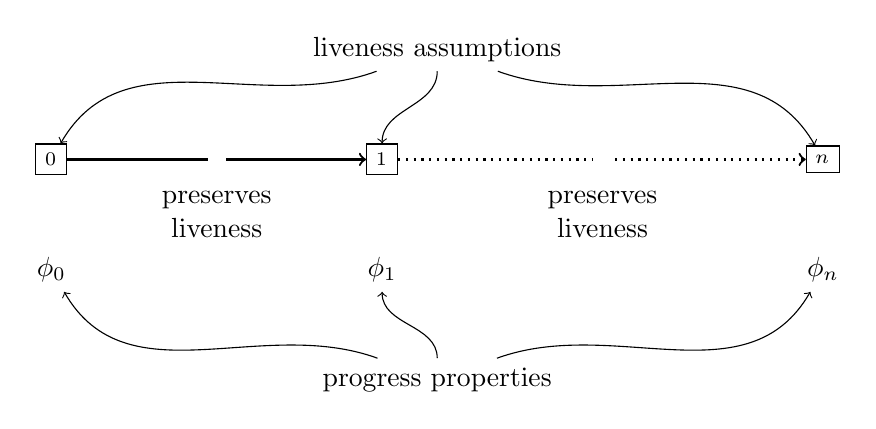
\begin{tikzpicture}[scale=1.4]
  \draw (0,0) node(m0)[align=center, draw]{$\Mch_0$};
  \draw (0,-0.5) node{\satisfies};
  \draw (0,-1) node(phi0){$\phi_0$};
  \draw (3,0) node(m1)[align=center, draw]{$\Mch_1$};
  \draw[->, thick] (m0) --node[align=center,fill=white]{\abstracts} (m1);
  \draw (3,-0.5) node{\satisfies};
  \draw (3,-1) node(phi1){$\phi_1$};
  \draw (7,0) node(mN)[align=center, draw]{$\Mch_n$};
  \draw[->, dotted, thick](m1) --node[align=center, fill=white]{\abstracts} (mN);
  \draw (7,-0.5) node{\satisfies};
  \draw (7,-1) node(phiN){$\phi_n$};

  \uncover<2->{
    \alert<2>{
      \draw (3.5, 1) node(asm){liveness assumptions};
      \draw[->] (asm) to[out=200, in=60] (m0);
      \draw[->] (asm) to[out=-90, in = 90] (m1);
      \draw[->] (asm) to[out=-20, in = 120] (mN);
    }
  }

  \uncover<3->{
    \alert<3>{
      \draw (3.5, -2) node(prg){progress properties};
      \draw[->] (prg) to[out=-200, in = -60] (phi0);
      \draw[->] (prg) to[out=90, in = -90] (phi1);
      \draw[->] (prg) to[out=20, in = -120] (phiN);
    }
  }

  \uncover<4->{
    \alert<4>{
      \draw (1.5, -0.5) node[align=center]{preserves\\liveness};
      \draw (5, -0.5) node[align=center]{preserves\\liveness};
    }
  }
\end{tikzpicture}

\ifx\PREAMBLE\UnDef
\end{document}
\else
\fi
